%!TEX root = htm.tex
\section{Hybrid Transactional Memory (HyTM)}
\label{sec:hytm}
%
\vspace{1mm}\noindent\textbf{Transactional Memory (TM).} 
A \emph{transaction} is a sequence of \emph{transactional operations}
(or \emph{t-operations}), reads and writes, performed on a set of \emph{transactional objects} 
(\emph{t-objects}). 
%Any transaction consists of \emph{transactional operations} (\emph{t-operations}) 
%consisting of an \emph{invocation} and a matching \emph{response}.
A TM \emph{implementation} provides a set of
concurrent \emph{processes} with deterministic algorithms that implement reads and
writes on t-objects using  a set of \emph{base objects}.
More precisely, for each transaction $T_k$, a TM implementation must support the following t-operations: 
$\mathit{read}_k(X)$, where $X$ is a t-object, that returns a value in
a domain $V$
or a special value $A_k\notin V$ (\emph{abort}),
$\mathit{write}_k(X,v)$, for a value $v \in V$,
that returns $\mathit{ok}$ or $A_k$, and
$\mathit{tryC}_k$ that returns $C_k\notin V$ (\emph{commit}) or $A_k$.
Additionally, we assume that a transaction $T_k$
may perform a $\mathit{start_k}$ that is the first t-operation performed by $T_k$ which returns $A_k$ or $\mathit{ok}$.
% \petrC{Is this start event necessary?}

\vspace{1mm}\noindent\textbf{Configurations and executions.} 
A \emph{configuration} of a TM implementation specifies the state of each base object and each process. 
In the \emph{initial} configuration, each base object has its initial value and each process is in its initial state. 
An \emph{event} (or \emph{step}) of a transaction invoked by some process is an invocation of a t-operation, 
a response of a t-operation, or an atomic \emph{primitive} operation applied to base object along with its response. 
%An event $e$ is \emph{applicable} to a configuration $C$ if $e$ can legally be applied to $C$. 
%Applying an event $e$ to a configuration $C$ results in another configuration $C' = e(C)$.
An \emph{execution fragment} is a (finite or infinite) sequence of events $E = e_1,e_2,\dots$. 
%$E$ is applicable to a configuration $C$ if $e_1$ is applicable to $C$, $e_2$ is applicable to $e_1(C)$, 
%and so forth. 
An \emph{execution} of a TM implementation $\mathcal{M}$ is an
execution fragment where, informally, each event respects the
specification of base objects and the algorithms specified by $\mathcal{M}$.
In the next section, we define precisely how base objects should
behave in a hybrid model combining direct memory accesses with \emph{cached} accesses (hardware
transactions).

%applicable to the initial configuration 
%where each event of each transaction is issued according to $\mathcal{M}$.
The \emph{read set} (resp., the \emph{write set}) of a transaction $T_k$ in an execution $E$,
denoted $\Rset_E(T_k)$ (and resp. $\Wset_E(T_k)$), is the set of t-objects that $T_k$ attempts to read (and resp. write) 
by issuing a t-read (and resp. t-write) invocation in $E$ (for brevity, we sometimes 
omit the subscript $E$ from the notation).
The \emph{data set} of $T_k$ is $\Dset(T_k)=\Rset(T_k)\cup\Wset(T_k)$.
$T_k$ is called \emph{read-only} if $\Wset(T_k)=\emptyset$; \emph{write-only} if $\Rset(T_k)=\emptyset$ and
\emph{updating} if $\Wset(T_k)\neq\emptyset$.
% Note that we consider the conventional dynamic TM model: 
% the data set of a transaction is identifiable only by the set of t-objects the transaction has invoked a read or write in the given execution.

For any finite execution $E$ and execution fragment $E'$, $E\cdot E'$ denotes the concatenation of $E$ and $E'$
and we say that $E\cdot E'$ is an \emph{extension}
of $E$.
%Let $E$ be an execution fragment.
For every transaction identifier $k$,
$E|k$ denotes the subsequence of $E$ restricted to events of
transaction $T_k$.
If $E|k$ is non-empty,
we say that $T_k$ \emph{participates} in $E$,
and let $\txns(E)$ denote the set of transactions that participate in $E$.
Two executions $E$ and $E'$
are \emph{indistinguishable} to a set $\mathcal{T}$ of transactions, if
for each transaction $T_k \in \mathcal{T}$, $E|k=E'|k$.

\vspace{1mm}\noindent\textbf{Complete and incomplete transactions.}
A transaction $T_k\in \txns(E)$ is \emph{complete in $E$} if
$E|k$ ends with a response event.
The execution $E$ is \emph{complete} if all transactions in $\txns(E)$
are complete in $E$.
A transaction $T_k\in \txns(E)$ is \emph{t-complete} if $E|k$
ends with $A_k$ or $C_k$; otherwise, $T_k$ is \emph{t-incomplete}.
$T_k$ is \emph{committed} (resp.\ \emph{aborted}) in $E$
if the last event of $T_k$ is $C_k$ (resp.\ $A_k$).
The execution $E$ is \emph{t-complete} if all transactions in
$\txns(E)$ are t-complete.
A configuration $C$ after an execution $E$ is \emph{quiescent} (resp. \emph{t-quiescent}) if 
every transaction $T_k \in \ms{txns}(E)$ is complete (resp. t-complete) in $E$.

\vspace{1mm}\noindent\textbf{Contention.}
%[[PK never used?
%Let $E\cdot e$ be a finite execution where $e$ is an event performed by transaction $T$.
%We then say that \emph{$T$ applies $e$ immediately after $E$}.
%]]
We assume that base objects are accessed with \emph{read-modify-write} (rmw) primitives. 
A rmw primitive $\langle g,h \rangle$ applied to a base object 
atomically updates the value of the object with a new value, which is
a function $g(v)$ of the old value $v$, and returns a response $h(v)$.
%A rmw primitive is \emph{trivial} if it never affects the value of a
%base object, otherwise it is \emph{nontrivial}.
A rmw primitive event on a base object is \emph{trivial} if, in any configuration, its application
does not change the state of the object. 
Otherwise, it is called \emph{nontrivial}.

Events $e$ and $e'$ of an execution $E$  \emph{contend} on a base
object $b$ if they are both primitives on $b$ in $E$ and at least 
one of them is nontrivial.
%We say that $e$ and $e'$ \emph{concurrently contend} on $b$ in $E$ if they contend on $b$ in the configuration $C$ after $E$.
In a configuration $C$ after an execution $E$, every incomplete transaction $T$  
has exactly one \emph{enabled} event in $C$, 
which is the next event $T$ will perform according to the TM implementation.
We say that a transaction $T$ is \emph{poised to apply an event $e$ after $E$} 
if $e$ is the next enabled event for $T$ in $E$.
We say that transactions $T$ and $T'$ \emph{concurrently contend on $b$ in $E$} 
if they are each poised to apply contending events on $b$ after $E$.
We say that an execution fragment $E$ is \emph{step contention-free} for t-operation $op_k$ if the events of $E|op_k$ 
are contiguous in $E$.
An execution fragment $E$ is \emph{step contention-free for $T_k$} if the events of $E|k$ are contiguous in $E$, and $E$ is \emph{step contention-free} if $E$ is step contention-free for all transactions that participate in $E$.

\vspace{1mm}\noindent\textbf{Direct accesses and cached accesses.}
We  now describe the execution model of a \emph{Hybrid Transactional Memory (HyTM)} implementation.
%, in which conventional memory accesses are combined with hardware
%transactions modelled as \emph{cached} accesses. 
%
In our HyTM model, every base object can be accessed with two kinds of
primitives, \emph{direct} and \emph{cached}.

In a direct access, the rmw primitive operates on the memory state:
the direct-access event atomically reads the value of the object in
the shared memory and, if necessary, modifies it.

In a cached access performed by a process $i$, the rmw primitive operates on the \emph{cached}
state recorded in process $i$'s \emph{tracking set} $\tau_i$. 
%[[PK unclear what ``initially'' means here
% (initially empty).  
%]]
One can think of $\tau_i$ as the \emph{L1 cache} of process $i$.
A \emph{hardware transaction}  is a series of cached rmw primitives performed on $\tau_i$ followed by
a \emph{cache-commit} primitive. 
 
More precisely, $\tau_i$ is a set of triples $(b, v, m)$ where $b$ is a base object identifier, $v$ is a value, 
and $m \in \{\shared, \exclusive\}$ is an access \emph{mode}. 
The triple $(b, v, m)$ is added to the tracking set when $i$ performs a cached
rmw access of $b$, where $m$ is set to $\exclusive$ if the access is
nontrivial, and to $\shared$ otherwise.  
We assume that there exists some constant $\TS$ (representing the size of the L1 cache)
such that the condition $|\tau_i| \leq \TS$ must always hold; this
condition will be enforced by our model.
A base object $b$ is \emph{present} in $\tau_i$ with mode $m$ if $\exists v, (b,v,m) \in \tau_i$.
%\petrC{Did not get what
%  ``enforced'' means here.}

%Like rmw primitives, a cached primitive is also characterized by the pair of update and response functions $\langle g,h \rangle$.
%Given a base object $b$ with value $v$ in a configuration $C$, 
A trivial (resp.\ nontrivial) 
cached primitive $\langle g,h \rangle$ applied to $b$ 
by process $i$ first checks the condition $|\tau_i|=\TS$ and if so, it
sets $\tau_i=\emptyset$ and immediately returns $\bot$ (we call this event a
\emph{capacity abort}). 
We assume that $\TS$ is large enough so that no transaction 
with data set of size $1$ can incur a capacity abort.
%
If the transaction does not incur a capacity abort, the process checks whether $b$ is present in exclusive
(resp.\ any) mode in $\tau_j$ 
for any $j\neq i$. If so, $\tau_i$ is set to $\emptyset$ and the
primitive returns $\bot$. 
%
Otherwise, the triple $(b, v, \shared)$ (resp. $(b, g(v), \exclusive)$)
is added to $\tau_i$,  where $v$ is the most recent cached value of $b$ in $\tau_i$
(in case $b$ was previously accessed by $i$ within the current
hardware transaction) or the value of $b$ in the current
memory configuration, and finally $h(v)$ is returned.
%

A tracking set can be \emph{invalidated} by a concurrent process: 
if, in a configuration $C$ where  $(b,v,\exclusive)\in\tau_i$
(resp.\ $(b,v,\shared)\in\tau_i)$,  a process $j\neq i$ applies any primitive 
(resp.\ any \emph{nontrivial} primitive) to $b$, then $\tau_i$ becomes
\emph{invalid} and any subsequent cached primitive invoked by $i$
sets $\tau_i$ to $\emptyset$ and returns $\bot$. We refer to this event as a \emph{tracking set abort}.

Finally, the \emph{cache-commit} primitive issued by process $i$ with
a valid $\tau_i$ does the following: for each base object $b$ such that $(b,v,\exclusive) \in \tau_i$, the value of $b$ in $C$ is updated to $v$. 
Finally, $\tau_i$ is set to $\emptyset$ and the primitive 
returns $\textit{commit}$. 

Note that HTM may also abort spuriously, or because of unsupported operations~\cite{Rei12}. 
The first cause can be modelled probabilistically in the above
framework, which would not however significantly affect our claims and proofs, except for a more cumbersome presentation. 
Also, our lower bounds are based exclusively on executions containing t-reads and t-writes. 
Therefore, in the following, we only consider tracking set and capacity aborts.  

\vspace{1mm}\noindent\textbf{Slow-path and fast-path transactions.}
In the following, we partition HyTM transactions into \emph{fast-path
  transactions} and \emph{slow-path transactions}.
Practically,  two separate algorithms (fast-path one and slow-path one) 
are provided for each t-operation. 

A slow-path transaction models a regular software transaction.
An event of a slow-path transaction is either an invocation or response of a t-operation, or
a  rmw primitive on a base object. 
% In further examples, we annotate fast-path transactions by $F$ and
% slow-path transactions by $S$. 

A fast-path transaction essentially encapsulates a hardware transaction. 
An event of a fast-path transaction is either an invocation or response of a t-operation, 
a cached primitive on a base object, or a \emph{cache-commit}:
\textit{t-read} and \emph{t-write} are only allowed to contain cached
primitives, and \textit{tryC} consists of invoking \emph{cache-commit}.  
Furthermore, we assume that a fast-path transaction $T_k$ returns $A_k$
as soon an underlying cached primitive or \emph{cache-commit} returns $\bot$. 

\textbf{Need to extend model to accomodate non-speculative operations}
We provide two key observations on this model regarding the interactions of non-committed fast path transactions 
with other transactions. 
Let $E$ be any execution of a HyTM implementation $\mathcal{M}$ in
which a fast-path transaction $T_k$ is either
t-incomplete or aborted. 
Then the sequence of events $E'$ derived by removing all events of $E|k$
from $E$ is an execution  $\mathcal{M}$. Moreover: 
%Then, the following observations are implied by our model.
\begin{observation} 
\label{ob:one}
To every slow-path transaction $T_m \in \ms{txns}(E)$, $E$ is indistinguishable 
from $E'$. 
\end{observation}
%
% \begin{figure*}[t]
% \begin{center}
% 	\subfloat[\label{sfig:ob-01}]{\scalebox{0.5}[0.5]{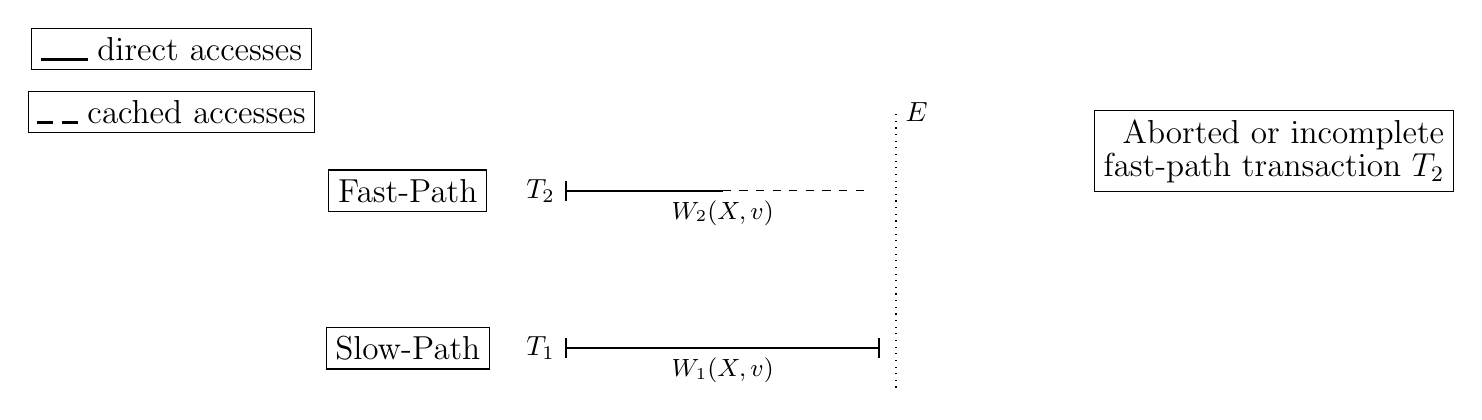
\begin{tikzpicture}
\node (w2) at (10,0) [] {};
\node (w1) at (10,-2) [] {};
\node (w3) at (18,-2) [] {};


\draw (w2) node [below] {\small {$W_2(X,v)$}};

\draw (w1) node [below] {\small {$W_1(X,v)$}};
%\draw (w1) node [below] {\tiny {$T_1$ commits}};

\node[draw,align=left] at (6,0) {{\large Fast-Path}};
\node[draw,align=left] at (6,-2) {{\large Slow-Path}};

\begin{scope}   
\draw [|-,thick] (8,0) node[left] {$T_2$} to (10,0);
\draw [-,dashed] (10,0) to (11.8,0);
\draw [|-|,thick] (8,-2) node[left] {$T_1$} to (12,-2);
\draw [-,dotted] (12.2,-2.5)  to (12.2,1) node[right] {$E$};
\end{scope}
%
\node[draw,align=right] at (17,.5) {\large {Aborted or incomplete}\\ {\large fast-path transaction $T_2$}};
%
\node[draw,align=right] at (3,1.8) {\rule{6mm}{1pt} \large {direct accesses}};
\node[draw,align=right] at (3,1) {\rule{2mm}{1pt} \rule{2mm}{1pt} \large{cached accesses}};

%
\end{tikzpicture}
}}
% 	\hspace{10mm}
% 	\subfloat[\label{sfig:ob-02}]{\scalebox{0.5}[0.5]{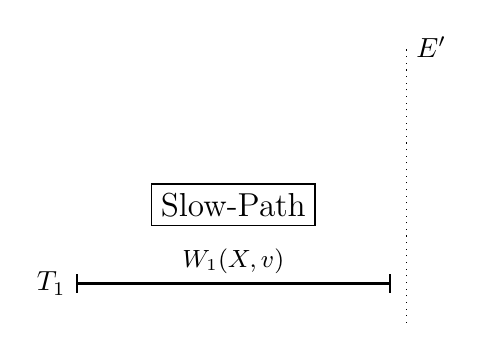
\begin{tikzpicture}

\node (w1) at (11,-2) [] {};


\draw (w1) node [above] {\small {$W_1(X,v)$}};
%\draw (w1) node [below] {\tiny {$T_1$ commits}};

\node[draw,align=left] at (11,-1) {{\large Slow-Path}};

\begin{scope}   
\draw [|-|,thick] (9,-2) node[left] {$T_1$} to (13,-2);
\draw [-,dotted] (13.2,-2.5)  to (13.2,1) node[right] {$E'$};
\end{scope}
%
%
\end{tikzpicture}
}}
% 	 
% \end{center}
% \caption{
% %Executions illustrating
%  %Observation~\ref{ob:one} 
%  \label{fig:ob1}
%  Execution $E$ in Figure~\ref{sfig:ob-01} is indistinguishable
% to $T_1$ from the execution $E'$ in Figure~\ref{sfig:ob-02}}
% \end{figure*}
%
\begin{observation} 
\label{ob:two}
If a fast-path transaction $T_m\in \ms{txns}(E) \setminus \{T_k\}$ does not incur a tracking set abort in $E$, 
then $E$ is indistinguishable to $T_m$ from $E'$.
\end{observation}
%
Intuitively, these observations say that fast-path transactions which are not yet committed are 
invisible to slow-path transactions, and can communicate with other
fast-path transactions only by incurring their tracking-set aborts.
